\documentclass[addpoints]{exam}

\usepackage{epic,array,ecltree,url}
\usepackage[nointegrals]{wasysym}


%These tell TeX which packages to use.
\usepackage{epsfig}
\usepackage{amsmath}
\usepackage{amsfonts}
\usepackage{amssymb}
\usepackage{amsxtra}
\usepackage{amsthm}
\usepackage{../mlextra} % must be below ams packages
\usepackage{mathrsfs}
\usepackage[dvipsnames]{xcolor}
\usepackage{array}
\usepackage{graphicx}
\graphicspath{ {../../art/} }
\usepackage{bm}
\usepackage{tikz}
\usepackage{multicol}

%Pagination stuff.
\setlength{\topmargin}{-.3 in}
\setlength{\oddsidemargin}{0in}
\setlength{\evensidemargin}{0in}
\setlength{\textheight}{9.in}
\setlength{\textwidth}{6.5in}

\newcommand{\twonode}{%
  \begingroup\normalfont
  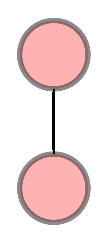
\includegraphics[height=\fontcharht\font`\b]{2nodetree.eps}%
  \endgroup
}

\newcommand{\tf}[1][{}]{%
\fillin[#1][0.25in]%
}
\noprintanswers
\unframedsolutions
\SolutionEmphasis{\itshape\small}
\SolutionEmphasis{\color{NavyBlue}}
\checkboxchar{$\Box$}
\checkedchar{$\blacksquare$}
\begin{document}


\noindent
\begin{tabular*}{\textwidth}{l @{\extracolsep{\fill}} r @{\extracolsep{6pt}} l}
{\large CS3001: Foundations of Computer Science} &  \makebox[3in]{\large Name:\enspace\hrulefill}\\
{\large May 13, 2019} & \\
{\large Quiz 3} & 
\end{tabular*}\\

\fbox{\fbox{\parbox{6in}{\textbf{Instructions}: Please answer the questions 
  below to the best of your ability. Be sure to show your work where appropriate. 
   This quiz is closed book, closed notes, closed computer. There are \numpoints\ 
   points in total. }}}\\

\begin{questions}
\question Let $A$ be the formula $(q \lor \ngg q) \imp (p \land \ngg p)$.

\begin{parts}
\part[2] Which of the following correctly characterize(s) $A$? (Choose all that apply) 

\begin{oneparcheckboxes}
\choice Valid
\choice Satisfiable
\CorrectChoice Falsifiable
\CorrectChoice Unsatisfiable
\end{oneparcheckboxes}
\vspace{2mm}

\part[2] Which of the following correctly characterize(s) $\ngg A$? (Choose all that apply) 

\begin{oneparcheckboxes}
\CorrectChoice Valid
\CorrectChoice Satisfiable
\choice Falsifiable
\choice Unsatisfiable
\end{oneparcheckboxes}
\vspace{2mm}
\end{parts}

\question[3] Let $A$ be the formula $(p \imp (\ngg (q \land p))) \lor (p \land q)$. Write $A$ in conjunctive normal form.
\vspace{30mm}
\begin{solution}
~\\
$(\ngg p \lor \ngg (q \land \ngg p)) \lor (p \land q)$\\
$(\ngg p \lor \ngg q \lor p) \lor (p \land q)$\\
$(\ngg p \lor \ngg q \lor p \lor p) \land (\ngg p \lor \ngg q \lor p \lor q)$\\
$(\ngg p \lor \ngg q \lor p) \land (\ngg p \lor \ngg q \lor p \lor q)$\\
\end{solution}

\question[2] Let $S$ be the formula $(x \imp y) \land \ngg (y \land \ngg x)$. Write $S$ in clausal notation.
\begin{solution}
~\\
$(x \imp y)\land \ngg (y \land \ngg x)$\\
$(\ngg x \lor y) \land (\ngg y \lor x)$\\
$\{\bar{x}y,x\bar{y}\}$\\
\end{solution}
\vspace{30mm}

\question[2] Let $A$ and $B$ be two problems such that $A \leq_{P} B$. Which of
the following can you conclude (choose all that apply)?
\begin{checkboxes}
\CorrectChoice If $A$ is NP-complete, $B$ is NP-Hard.
\choice If $A$ is in $P$, $B$ is in NP. 
\CorrectChoice If $B$ is decidable, $A$ is also decidable.
\CorrectChoice $B$ is at least as hard as $A$.
\end{checkboxes}

\vspace{10mm}
\question[2] Let $S = S_0 = \{t,rs\bar{t},\bar{u}\bar{v},uv\}$. Following the resolution
procedure discussed in class, which of the following are possible correct
values of $S_1$ (choose all that apply)?
\begin{checkboxes}
\CorrectChoice $S_1 = \{t,rs\bar{t},\bar{u}\bar{v},uv, rs\}$ 
\choice $S_1 = \{t,rs\bar{t},\bar{u}\bar{v},uv, \Box \}$ 
\choice $S_1 = \{rs,\bar{u}\bar{v},uv\}$ 
\CorrectChoice $S_1 = \{t,rs\bar{t},\bar{u}\bar{v},uv\}$ 
\end{checkboxes}


\vspace{5mm}

\end{questions}
\end{document}


